\documentclass[conference,a4paper]{IEEEtran}
\pdfobjcompresslevel=0
\IEEEoverridecommandlockouts
% The preceding line is only needed to identify funding in the first footnote. If that is unneeded, please comment it out.
%Template version as of 6/27/2024

\usepackage{cite}
\usepackage{amsmath,amssymb,amsfonts}
\usepackage{algorithmic}
\usepackage{graphicx}
\usepackage{url}
\usepackage{textcomp}

\usepackage{multirow}
% --- packages required by this paper's full-width floats and barriers ---
\usepackage{dblfloatfix}
\usepackage{placeins}
\usepackage{float}
\def\BibTeX{{\rm B\kern-.05em{\sc i\kern-.025em b}\kern-.08em
    T\kern-.1667em\lower.7ex\hbox{E}\kern-.125emX}}

% --- float tuning to keep the paper within the page limit ---
\setcounter{topnumber}{2}
\setcounter{dbltopnumber}{3}
\renewcommand{\topfraction}{0.9}
\renewcommand{\dbltopfraction}{0.9}
\renewcommand{\textfraction}{0.07}
\renewcommand{\floatpagefraction}{0.85}
\renewcommand{\dblfloatpagefraction}{0.92}
\setlength{\textfloatsep}{6pt plus 1pt minus 2pt}
\setlength{\floatsep}{6pt plus 1pt minus 2pt}
\setlength{\intextsep}{6pt plus 1pt minus 2pt}
\setlength{\abovecaptionskip}{2pt}
\setlength{\belowcaptionskip}{0pt}

\begin{document}
\raggedbottom

\title{A POMDP-Based Framework for Healthcare Decision-Making
to Mitigate Cognitive Decline in Alzheimer's Disease}

\author{%
\IEEEauthorblockN{1\textsuperscript{st} Ahmad Alfan Alfian Irfan}
\IEEEauthorblockA{\textit{Department of Information Technology} \\
\textit{Universitas Muhammadiyah Yogyakarta} \\
Yogyakarta, Indonesia \\
ahmad.alfan.ft23@mail.umy.ac.id}
\and
\IEEEauthorblockN{2\textsuperscript{nd} Slamet Riyadi}
\IEEEauthorblockA{\textit{Department of Information Technology} \\
\textit{Universitas Muhammadiyah Yogyakarta} \\
Yogyakarta, Indonesia \\
Corresponding email: riyadi@umy.ac.id}
}
\maketitle

\begin{abstract}
Alzheimer's disease staging involves sequential decisions from noisy
clinical evidence. We formulate this process as a Partially Observable
Markov Decision Process (POMDP), combining components estimated from the
Alzheimer's Disease Neuroimaging Initiative (ADNI) with explicit modeling
assumptions. The contributions are a benchmark with traceable parameter
provenance, a comparison of four policy classes, and interpretation of
the offline policy through belief-space decision regions. Across 100,000
simulated episodes per policy, SARSOP achieves the highest mild cognitive
impairment (MCI) intake-stage agreement (81.2\%) and lowest testing
expenditure among informed policies. MyopicPOMDP achieves the highest
Dementia intake-stage agreement (87.3\%) without offline planning.
Their episode-weighted overall accuracies are 78.3\% and 78.1\%,
respectively, while equal-stage macro accuracies are 76.6\% and 79.8\%.
Reward comparisons are conditional on the stopping protocol. Transition
dynamics, initial beliefs, and APOE4 likelihoods are ADNI-derived;
Mini-Mental State Examination (MMSE), Clinical Dementia Rating (CDR)
likelihoods, and utilities are hand-specified. The results characterize
simulated management decisions. Biological mitigation of cognitive
decline remains an intended application rather than a demonstrated outcome.
\end{abstract}

\begin{IEEEkeywords}
POMDP, Alzheimer's disease, ADNI, healthcare decision-making,
clinical decision support, SARSOP, belief state, cognitive decline
\end{IEEEkeywords}

\section{Introduction}

Global dementia prevalence was estimated at 57.4 million in 2019 and
projected to reach 152.8 million by 2050~\cite{nichols2022}.
Alzheimer's disease (AD) is a major cause of dementia. We represent
clinical status as Cognitively Normal (CN), Mild Cognitive Impairment
(MCI), or Dementia. CN denotes age-expected cognitive performance;
MCI denotes impairment without substantial loss of independence;
Dementia denotes impairment that disrupts independent living.
Monitoring MCI supports reassessment and management
planning~\cite{petersen2018mci}. Available evidence includes the
30-point Mini-Mental State Examination (MMSE) cognitive
screen~\cite{folstein1975mmse}, the Clinical Dementia Rating (CDR)
functional assessment~\cite{hughes1982cdr}, and the APOE4 genetic
risk marker~\cite{corder1993apoe}. These instruments provide
different, imperfect information about clinical status.

Computational approaches support AD assessment through stage
classification from acquired measurements~\cite{wen2020convolutional}
and prediction of future conversion~\cite{grueso2021machine}.
These tasks provide useful estimates, but a prediction alone does not
determine which additional assessment to obtain or when the available
evidence warrants a management decision. In a sequential workflow,
another test incurs a cost and can change the preferred action,
while premature commitment risks a stage-inappropriate decision.
The problem addressed here is therefore not only to estimate clinical
stage, but to decide whether further information is worth acquiring.

A Partially Observable Markov Decision Process
(POMDP) represents this problem by separating the latent clinical
state from its noisy observations~\cite{kaelbling,cassandra}.
It maintains a probability distribution, or belief, over stages and
updates that distribution as evidence arrives. The policy compares
the expected utility of a management commitment with the value of
additional testing~\cite{hauskrecht,monahan}. Testing cost, uncertainty,
and the consequences of an incorrect commitment thus enter a common
decision objective. This formulation can also inform future
connected-health workflows with intermittent
measurements~\cite{arrayyan2024iomt}; the present study evaluates the
decision model, not a deployed monitoring system.

Prior decision-theoretic studies examine preclinical AD
screening~\cite{onendumlu}, dementia subtype
differentiation~\cite{navarro}, and diagnostic and treatment choices
in acute stroke~\cite{khatim}. We investigate a complementary
combination of CN--MCI--Dementia staging, multi-test selection, and
management commitment, asking how policy choice changes stage
agreement, testing expenditure, and commitment timing.
Anticipation refers to utility-dependent commitment under uncertainty
rather than demonstrated prediction of future decline. Mitigation
is the intended healthcare application, not an established treatment
effect: management actions end the simulated episode and do not
alter disease progression.

The study makes three contributions. First, it separates the initial
belief, transition dynamics, and APOE4 likelihoods estimated from the
Alzheimer's Disease Neuroimaging Initiative (ADNI) cohort
from hand-specified MMSE/CDR likelihoods and decision utilities.
Second, it compares Random, Expert, MyopicPOMDP, and SARSOP under
a shared evaluation protocol, exposing subgroup and cost trade-offs.
Third, it extracts the SARSOP policy into inspectable belief regions
to characterize commitment decisions. Project code is available at
\url{https://github.com/PannnTastic/AnticipAD}.

\section{Related Work}

\subsection{Alzheimer's Disease and Clinical Staging}
\label{subsec:ad}
AD pathology can precede clinical symptoms by
years~\cite{jack2010hypothetical,sperling2011preclinical}.
ADNI links repeated cognitive assessments, imaging, and genetic
markers~\cite{petersen2010adni,jack2008adni,mueller2005adni}, supporting
classification and conversion-prediction
studies~\cite{wen2020convolutional,grueso2021machine}.
Using MMSE/CDR to estimate likelihoods against diagnoses partly
defined by those scores introduces incorporation bias.
Hand-specified likelihoods expose this assumption but do not
establish independent diagnostic validity.

\subsection{Partially Observable Markov Decision Processes}
\label{subsec:pomdp}
A POMDP comprises hidden states $\mathcal{S}$, actions $\mathcal{A}$,
observations $\mathcal{O}$, transition probabilities $T$, observation
likelihoods $Z$, rewards $R$, and discount factor
$\gamma\in[0,1)$~\cite{kaelbling,smallwood}. A belief distribution is
updated after each action and observation, and a policy maps that
belief to an action~\cite{monahan}. Exact planning is generally
intractable~\cite{cassandra}; point-based methods plan on selected
beliefs~\cite{pineau}, with SARSOP emphasizing reachable
regions~\cite{kurniawati}. POMCP and DESPOT instead use online
search~\cite{silver,ye}. Our reported comparison uses two baselines,
one-step lookahead, and offline point-based planning through
POMDPs.jl~\cite{egorov2017pomdps}.

\subsection{Sequential Medical Decision Support}
\label{subsec:medical}
Decision-theoretic clinical systems include treatment planning and
allocation models~\cite{hauskrecht,ahn}; more recent reinforcement
learning studies examine test acquisition and
stopping~\cite{yu2023drl,bernardino2022rl,meng2025costeffective}.
For AD, {\"O}nen Duml{\"u} et al.~\cite{onendumlu} consider
preclinical screening, while Navarro Posada~\cite{navarro} studies
dementia subtype differentiation. Khatim et al.~\cite{khatim}
integrate diagnostic observations and treatment decisions for stroke.

Our contribution combines chronic staging, multiple assessment
channels, management commitments, and policy interpretation.
It complements these prior formulations by examining how policy
choice changes intake-stage agreement, testing expenditure, and
commitment timing. This is an application and evaluation contribution;
the underlying planning algorithms are established methods.

\section{POMDP Model}

We define the POMDP as $\langle \mathcal{S}, \mathcal{A}, \mathcal{O},
T, Z, R, \gamma, b_0 \rangle$ with discount factor $\gamma = 0.95$.
A discount of $0.95$ places strong weight on future rewards while
penalizing unnecessary delays.
The evaluation cap, $H=20$ decision epochs, was chosen to match the
maximum number of visit records per participant in the assembled ADNI
dataset before listwise exclusion (15,836 records; 3,777 participants).
After removing records missing diagnosis or MMSE, the maximum is 19;
the cap retains the original dataset-based value of 20.
This choice bounds testing by the longest available visit sequence,
not a clinically optimal duration or SARSOP's planning horizon.
Each non-terminal test represents one modeled follow-up visit with
one selected assessment. Because preprocessing pools consecutive
visits without standardizing their elapsed time, an epoch has units
of visits, not a calibrated six-month duration. Consequently, $H=20$
does not establish a ten-year follow-up period. Sensitivity to
alternative caps remains untested.

\subsection{ADNI Calibration and State Space}

The disease-progression parameters, the APOE4 likelihoods, and the
initial belief are estimated from the ADNI 1/GO/2/3 merged
cohort~\cite{petersen2010adni,jack2008adni,mueller2005adni}, whereas the
MMSE and CDR likelihoods are hand-specified clinical models
(Table~\ref{tab:model}) rather than population-representative
frequencies. The calibration followed a stepwise cleaning process.

We started by extracting visit diagnoses from the \texttt{ADNIMERGE2}
diagnosis field. We then excluded non-Alzheimer etiologies and the
Significant Memory Concern category, and merged early MCI into MCI
to align the labels with our three-stage state space. That filtering
step yielded 15,836 visit records from 3,777 participants, with missing values coded as \texttt{NA}. We next
removed records missing either the diagnosis or the MMSE score
listwise, leaving 12,464 records for the prior and transition
estimates. No imputation was applied. The ADNI-derived APOE4
likelihoods were computed from observed values only. For modeling, MMSE scores
were grouped into Normal ($>$24), Moderate (20--24), and Low ($<$20),
CDR scores into 0, 0.5, and $\geq$1, and APOE4 into Negative,
Heterozygous, and Homozygous.

The latent state space is $\mathcal{S} = \{\mathrm{CN}, \mathrm{MCI},
\mathrm{Dementia}\}$. The initial belief is estimated from the
visit-level stage frequencies in the 12,464 retained records:
\begin{equation}
b_0 = [0.385,\; 0.417,\; 0.198].
\label{eq:prior}
\end{equation}
In \eqref{eq:prior}, the entries are dimensionless probabilities in
CN, MCI, Dementia order. Each $b_0(s)$ lies in $[0,1]$
(0--100\%) and the entries sum to one; the smallest and largest
specified entries are 0.198 and 0.417. These proportions correspond to 4,801 CN, 5,198 MCI, and 2,465 Dementia
records from 3,713 unique participants, so $b_0$ represents the
empirical stage mixture after listwise exclusion, not a patient-intake prior.

The six actions comprise three tests and three terminal commitments.
\textit{MMSE}, \textit{CDR}, and \textit{APOE4} incur testing costs
and return categorical observations without ending the episode.
For each test, the simulator advances the latent state by one visit
transition, then samples the result conditional on the updated state.
\textit{Wait} commits to routine surveillance without active treatment,
\textit{TreatMCI} to structured monitoring and care planning, and
\textit{TreatDem} to dementia management. These commitments end the
episode; their clinical consequences are not simulated.

\subsection{Transition, Observation, and Reward Parameters}

Table~\ref{tab:model} reports the transition, observation, and reward
parameters. Transition frequencies are estimated from consecutive
same-participant records after sorting by visit date, without
interval filtering or time rescaling. Dementia is then made absorbing
and MCI-to-CN reversion is fixed at zero. Only the selected test produces
an informative observation, which means that the actions Wait, TreatMCI,
and TreatDem return a null observation. The APOE4 likelihoods are estimated from ADNI frequencies,
whereas the MMSE and CDR likelihoods are hand-specified clinical noise
models, because diagnostic labels partly incorporate these instruments.
Their original descriptions motivate cognitive and functional
assessment~\cite{folstein1975mmse,hughes1982cdr}; they do not establish
the specific likelihood values in Table~\ref{tab:model}. CDR achieves a 90-percentage-point
separation between CN and Dementia (95\% vs.\ 5\% for CDR$=0$), compared
with 65 percentage points for MMSE (85\% vs.\ 20\% Normal), making CDR
more discriminative under these assumptions. APOE4 encodes genetic risk rather than
direct staging evidence. The reward function encodes a clinical preference
ordering: the $-1000$ penalty for waiting in Dementia captures the cost of
failing to recognize advanced disease, while the $-500$ penalty for TreatDem
in a CN patient guards against overtreatment. These dimensionless utility
points express decision preferences, not monetary costs or
clinically validated treatment benefits. Single-action rewards range
from $-1000$ to $+300$. Sensitivity checks in Section~\ref{sec:sensitivity}
assess selected assumptions; they do not calibrate these utilities.

\begin{table}[!t]
\caption{Model parameters. All probabilities are dimensionless.
$T$ and APOE4 are ADNI-derived with structural constraints; MMSE,
CDR, and utilities are hand-specified. $\gamma=0.95$; $H=20$.}
\label{tab:model}
\centering
\footnotesize
\setlength{\tabcolsep}{4pt}
\renewcommand{\arraystretch}{1.05}
\begin{tabular}{lrrr}
\hline
Visit transitions & CN & MCI & Dementia\\
\hline
From CN       & 0.929 & 0.068 & 0.003\\
From MCI      & 0     & 0.892 & 0.108\\
From Dementia & 0     & 0     & 1\\
\hline
Observation given stage & CN & MCI & Dementia\\
\hline
MMSE Normal ($>24$)   & 0.85 & 0.55 & 0.20\\
MMSE Moderate (20--24)& 0.13 & 0.35 & 0.45\\
MMSE Low ($<20$)      & 0.02 & 0.10 & 0.35\\
CDR 0                & 0.95 & 0.25 & 0.05\\
CDR 0.5              & 0.04 & 0.70 & 0.30\\
CDR $\geq1$          & 0.01 & 0.05 & 0.65\\
APOE4 Negative       & 0.69 & 0.56 & 0.34\\
APOE4 Heterozygous   & 0.28 & 0.35 & 0.47\\
APOE4 Homozygous     & 0.03 & 0.09 & 0.19\\
\hline
Action utility (points) & CN & MCI & Dementia\\
\hline
Wait    & $+30$ & $-10$ & $-1000$\\
MMSE    & $-5$ & $-5$ & $-5$\\
CDR     & $-20$ & $-20$ & $-20$\\
APOE4   & $-50$ & $-50$ & $-50$\\
TreatMCI& $-50$ & $+150$ & $-50$\\
TreatDem& $-500$ & $-100$ & $+300$\\
\hline
\end{tabular}
\end{table}

\subsection{Belief Update}

After an action $a$ produces observation $o$, the belief is updated by
Bayes' rule:
\begin{equation}
b'(s') = \eta\, Z(o \mid s', a)\sum_s T(s' \mid s, a)\, b(s),
\label{eq:belief}
\end{equation}
In \eqref{eq:belief}, $s,s'\in\mathcal{S}$ denote the current and
next latent stages, $a\in\mathcal{A}$ the selected action, and
$o\in\mathcal{O}$ its categorical result. The probabilities $b(s)$
and $b'(s')$ describe the prior and updated beliefs.
$T(s'\mid s,a)$ is the one-interval transition probability and
$Z(o\mid s',a)$ the observation likelihood. The normalization is
$\eta=1/P(o\mid b,a)$, where
$P(o\mid b,a)=\sum_{s'}Z(o\mid s',a)\sum_sT(s'\mid s,a)b(s)>0$.
All probabilities are dimensionless, lie in $[0,1]$, and normalize
over their respective outcomes. Policies use this same update rule;
their chosen tests and observed histories can nevertheless differ.

\section{Policies and Evaluation Protocol}

\textbf{Random} samples uniformly from the six actions and serves as an
uninformed baseline. \textbf{Expert} applies fixed clinical
thresholds ($p_\mathrm{CN}\geq0.80$, $p_\mathrm{MCI}\geq0.80$,
$p_\mathrm{Dem}\geq0.85$) and otherwise tests in a fixed
MMSE--CDR--APOE4 order. \textbf{MyopicPOMDP} performs a one-step
Bayesian lookahead without training. For a candidate test
$a_\mathrm{test}$, its stage-independent immediate expected reward is
\begin{equation}
C(b, a_\mathrm{test}) = \sum_s b(s)\,R(s, a_\mathrm{test}),
\label{eq:myopic_cost}
\end{equation}
and its discounted expected terminal value is
\begin{equation}
\begin{aligned}
V(b,a_\mathrm{test})={}&\gamma\sum_o P(o\mid b,a_\mathrm{test})\\
&{}\times\max_{a'\in\mathcal{A}_\mathrm{term}}
\sum_{s'}b'_o(s')R(s',a').
\end{aligned}
\label{eq:myopic_val}
\end{equation}
Here $C$ in \eqref{eq:myopic_cost} is the immediate expected test
reward, $V$ in \eqref{eq:myopic_val} is the discounted expected
terminal reward, $a_\mathrm{test}$ is a candidate test, and
$a'$ is a candidate terminal action. $R(s,a)$ is the utility in
Table~\ref{tab:model}; $\gamma=0.95$ is dimensionless. The observation
probability is defined after \eqref{eq:belief}, $b'_o$ is its updated
belief, and
$\mathcal{A}_\mathrm{term} = \{\mathrm{Wait},\mathrm{TreatMCI},
\mathrm{TreatDem}\}$ is the set of terminal commitment actions. The
total one-step value of the test action is then the sum of the two
terms,
\begin{equation}
Q(b, a_\mathrm{test}) = C(b, a_\mathrm{test}) + V(b, a_\mathrm{test}),
\label{eq:myopic}
\end{equation}
The test value $Q$ in \eqref{eq:myopic} is compared with the immediate
terminal values $Q(b,a')=\sum_s b(s)R(s,a')$; the maximizing action
is selected. $C$, $V$, and $Q$ are measured in the same utility points.

\textbf{SARSOP}~\cite{kurniawati} is an offline point-based solver that
precomputes $\alpha$-vectors over the reachable belief space and selects
actions by value lookup during simulation. All experiments are
implemented in Julia using the POMDPs.jl
ecosystem~\cite{egorov2017pomdps}.

Each solver is evaluated across ten random seeds with $N=10{,}000$
episodes per seed, for 100,000 episodes per policy. An episode starts
with a latent intake stage sampled from $b_0$. Test actions update the
stage and belief; a terminal action ends the episode. After $H=20$
non-terminal tests, the implementation appends a fallback Wait
commitment, so the recorded action count can reach 21. SARSOP
training required approximately 300\,s (requested precision $10^{-2}$,
timeout 300\,s); this requested tolerance does not itself certify
optimality. The stored policy was planned on a continuing model,
whereas evaluation stops at commitment, which limits optimality-based
comparisons with MyopicPOMDP.

For each seed, let $n_s$ be the number of episodes with intake stage
$s$, $c_s$ the number whose terminal action matches that stage, and
$N=\sum_s n_s=10{,}000$. The reported metrics are
\begin{equation}
\begin{aligned}
\mathrm{Acc}_s &= 100\,c_s/n_s,\\
\mathrm{Acc}_{\mathrm{overall}} &= 100\,\sum_s c_s/N,\\
\mathrm{Acc}_{\mathrm{macro}} &= \tfrac{1}{3}\sum_s\mathrm{Acc}_s .
\end{aligned}
\label{eq:accuracy}
\end{equation}
All accuracies in \eqref{eq:accuracy} range from 0 to 100\%.
Overall accuracy weights stages by their realized episode counts;
macro accuracy weights the three stages equally. Table~\ref{tab:bench}
reports means and sample standard deviations across ten seeds.

Correct intake-stage commitments are Wait for CN, TreatMCI for MCI,
and TreatDem for Dementia. Fixing the intake label preserves a common
reference across policies with different stopping times. This endpoint
measures agreement with the presenting stage, not the appropriateness
of management at commitment: an initially MCI case that progresses to
Dementia and receives TreatDem is scored incorrect against intake.
Consequently, these metrics cannot establish contemporaneous diagnostic
accuracy or treatment efficacy. Reward uses the evolving pre-action
state and a discount of $\gamma^{t-1}$ at decision $t$, including a
fallback commitment when needed. Testing cost sums undiscounted test
utilities; mean decisions counts tests and the terminal action.

\section{Results}
\label{sec:results}

\subsection{Benchmark Performance}

\begin{figure}[!t]
\centering
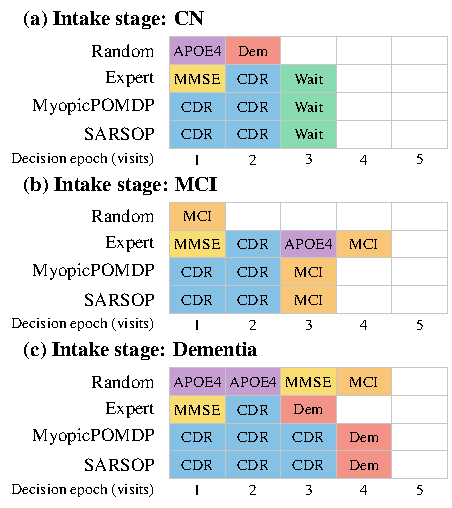
\includegraphics[width=\columnwidth]{figures/fig1_actions_revised.pdf}
\caption{Illustrative action sequences for simulated intake stages CN,
MCI, and Dementia. The x-axis counts decision visits, starting at
intake ($t=1$); visits are not calibrated calendar intervals. Blank
cells follow termination. Only the first five epochs are shown because
all displayed sequences terminate by epoch 4.}
\label{fig:traj}
\end{figure}

\begin{table*}[htbp]
\caption{Solver performance (mean $\pm$ SD across 10 seeds, 10,000 episodes each).
Accuracies score intake-stage agreement; overall accuracy is episode-weighted.
Reward and test cost are utility points. Bold marks the best column value,
including the smallest decision count and least negative testing cost.}
\label{tab:bench}
\begin{center}
\begin{tabular}{|l|c|c|c|c|c|c|c|}
\hline
Policy & Reward & CN Acc.\,(\%) & MCI Acc.\,(\%) & Dem.\ Acc.\,(\%) &
Overall Acc.\,(\%) & Cumul.\ Test Cost & Mean Decisions \\
\hline
SARSOP      & $68.7{\pm}1.5$ &
$80.4{\pm}0.7$ & $\mathbf{81.2{\pm}0.6}$ & $68.2{\pm}1.3$ &
$\mathbf{78.3{\pm}0.4}$ & $-29.9{\pm}0.1$ & $2.50{\pm}0.01$ \\
MyopicPOMDP & $\mathbf{73.0{\pm}1.2}$ &
$\mathbf{80.5{\pm}0.4}$ & $71.4{\pm}0.6$ & $\mathbf{87.3{\pm}0.7}$ &
$78.1{\pm}0.3$ & $-37.3{\pm}0.1$ & $2.87{\pm}0.01$ \\
Expert      & $44.7{\pm}1.9$ &
$79.8{\pm}0.6$ & $61.3{\pm}0.5$ & $75.1{\pm}1.0$ &
$71.1{\pm}0.4$ & $-42.1{\pm}0.4$ & $3.34{\pm}0.01$ \\
Random      & $-134.9{\pm}4.4$ &
$33.5{\pm}0.6$ & $33.3{\pm}0.8$ & $33.3{\pm}1.1$ &
$33.4{\pm}0.5$ & $\mathbf{-25.1{\pm}0.4}$ & $\mathbf{2.01{\pm}0.01}$ \\
\hline
\end{tabular}
\end{center}
\end{table*}

Fig.~\ref{fig:traj} shows the qualitative behavior on representative
patients, where colors encode actions: Wait (green), MMSE (yellow),
CDR (blue), APOE4 (purple), TreatMCI (orange), and TreatDem (red);
blank cells indicate epochs after the episode has ended. These selected
examples illustrate short test sequences and terminal commitments;
Random also terminates but can select an inappropriate action.

Table~\ref{tab:bench} reports the main results using episode-weighted
overall accuracy from \eqref{eq:accuracy}. Both belief-driven policies
improve overall intake-stage accuracy and reward over Expert and Random,
but do not dominate every subgroup or efficiency measure. SARSOP has
lower Dementia accuracy than Expert, while Random has the lowest
testing expenditure and fewest decisions. Equal stage weighting gives
macro accuracies of $76.6\pm0.5\%$ (SARSOP), $79.8\pm0.3\%$
(MyopicPOMDP), $72.1\pm0.5\%$ (Expert), and $33.4\pm0.6\%$ (Random),
computed per seed before aggregation.
Across the ten shared seeds, every headline contrast is
significant under a two-sided paired Wilcoxon signed-rank test with Holm
correction ($p<0.05$): SARSOP exceeds MyopicPOMDP in MCI accuracy by
$9.8$\,pp, MyopicPOMDP exceeds SARSOP in Dementia accuracy by $19.1$\,pp,
and MyopicPOMDP exceeds SARSOP in aggregate reward by $4.3$
(95\% CI $[3.8,4.8]$, Cliff's $\delta{=}1.0$). The reward advantage
is partly an effect of the terminate-at-first-commitment protocol;
the ranking is not a single-seed artifact. Since each seed already aggregates $N=10{,}000$ episodes,
this test assesses the \emph{stability} of the ranking across seeds
rather than a clinical effect size, which would require outcome data
external to the simulation.

Fig.~\ref{fig:rewarddist} separates reward by intake stage. The
contrasting MCI and Dementia distributions complement the intake
accuracies in Table~\ref{tab:bench}; aggregate reward alone conceals
these subgroup differences.

\begin{figure*}[!t]
\centering
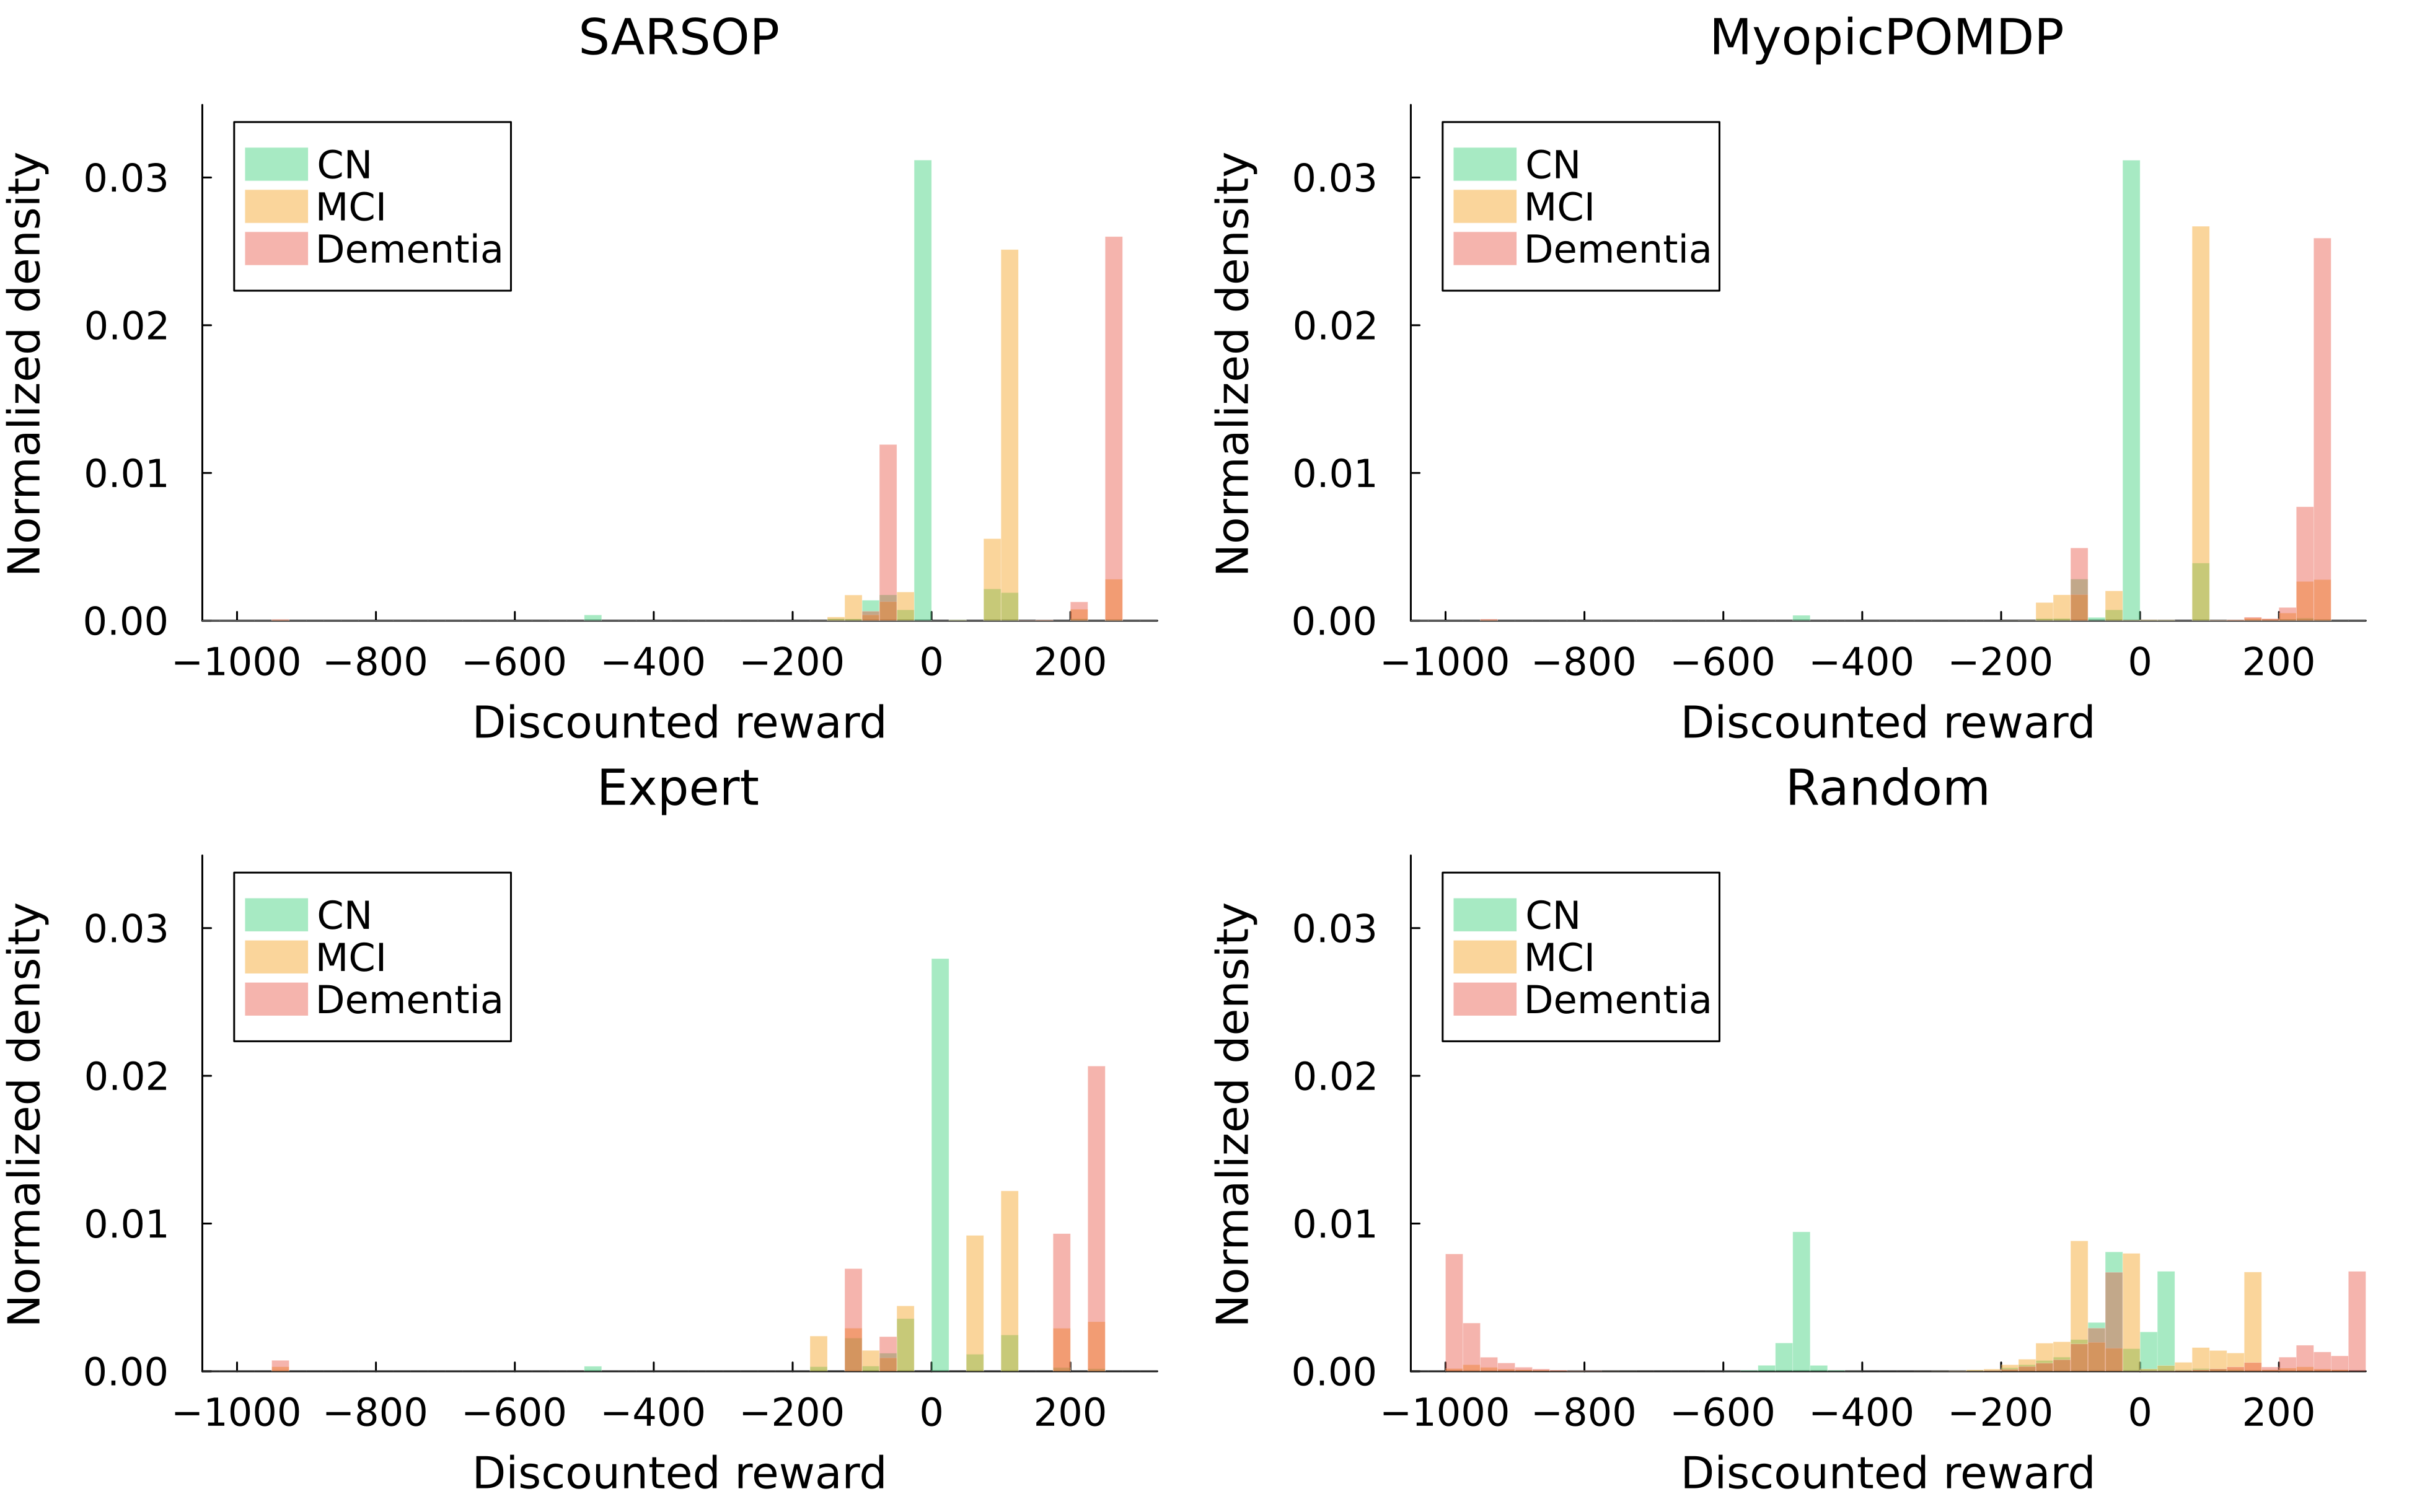
\includegraphics[width=0.76\textwidth]{figures/fig_reward_distribution_by_state.png}
\caption{Discounted reward distributions by intake stage and policy.
The x-axis is in dimensionless utility points; density on the y-axis
is per utility point.}
\label{fig:rewarddist}
\end{figure*}

\begin{figure*}[!t]
\centering
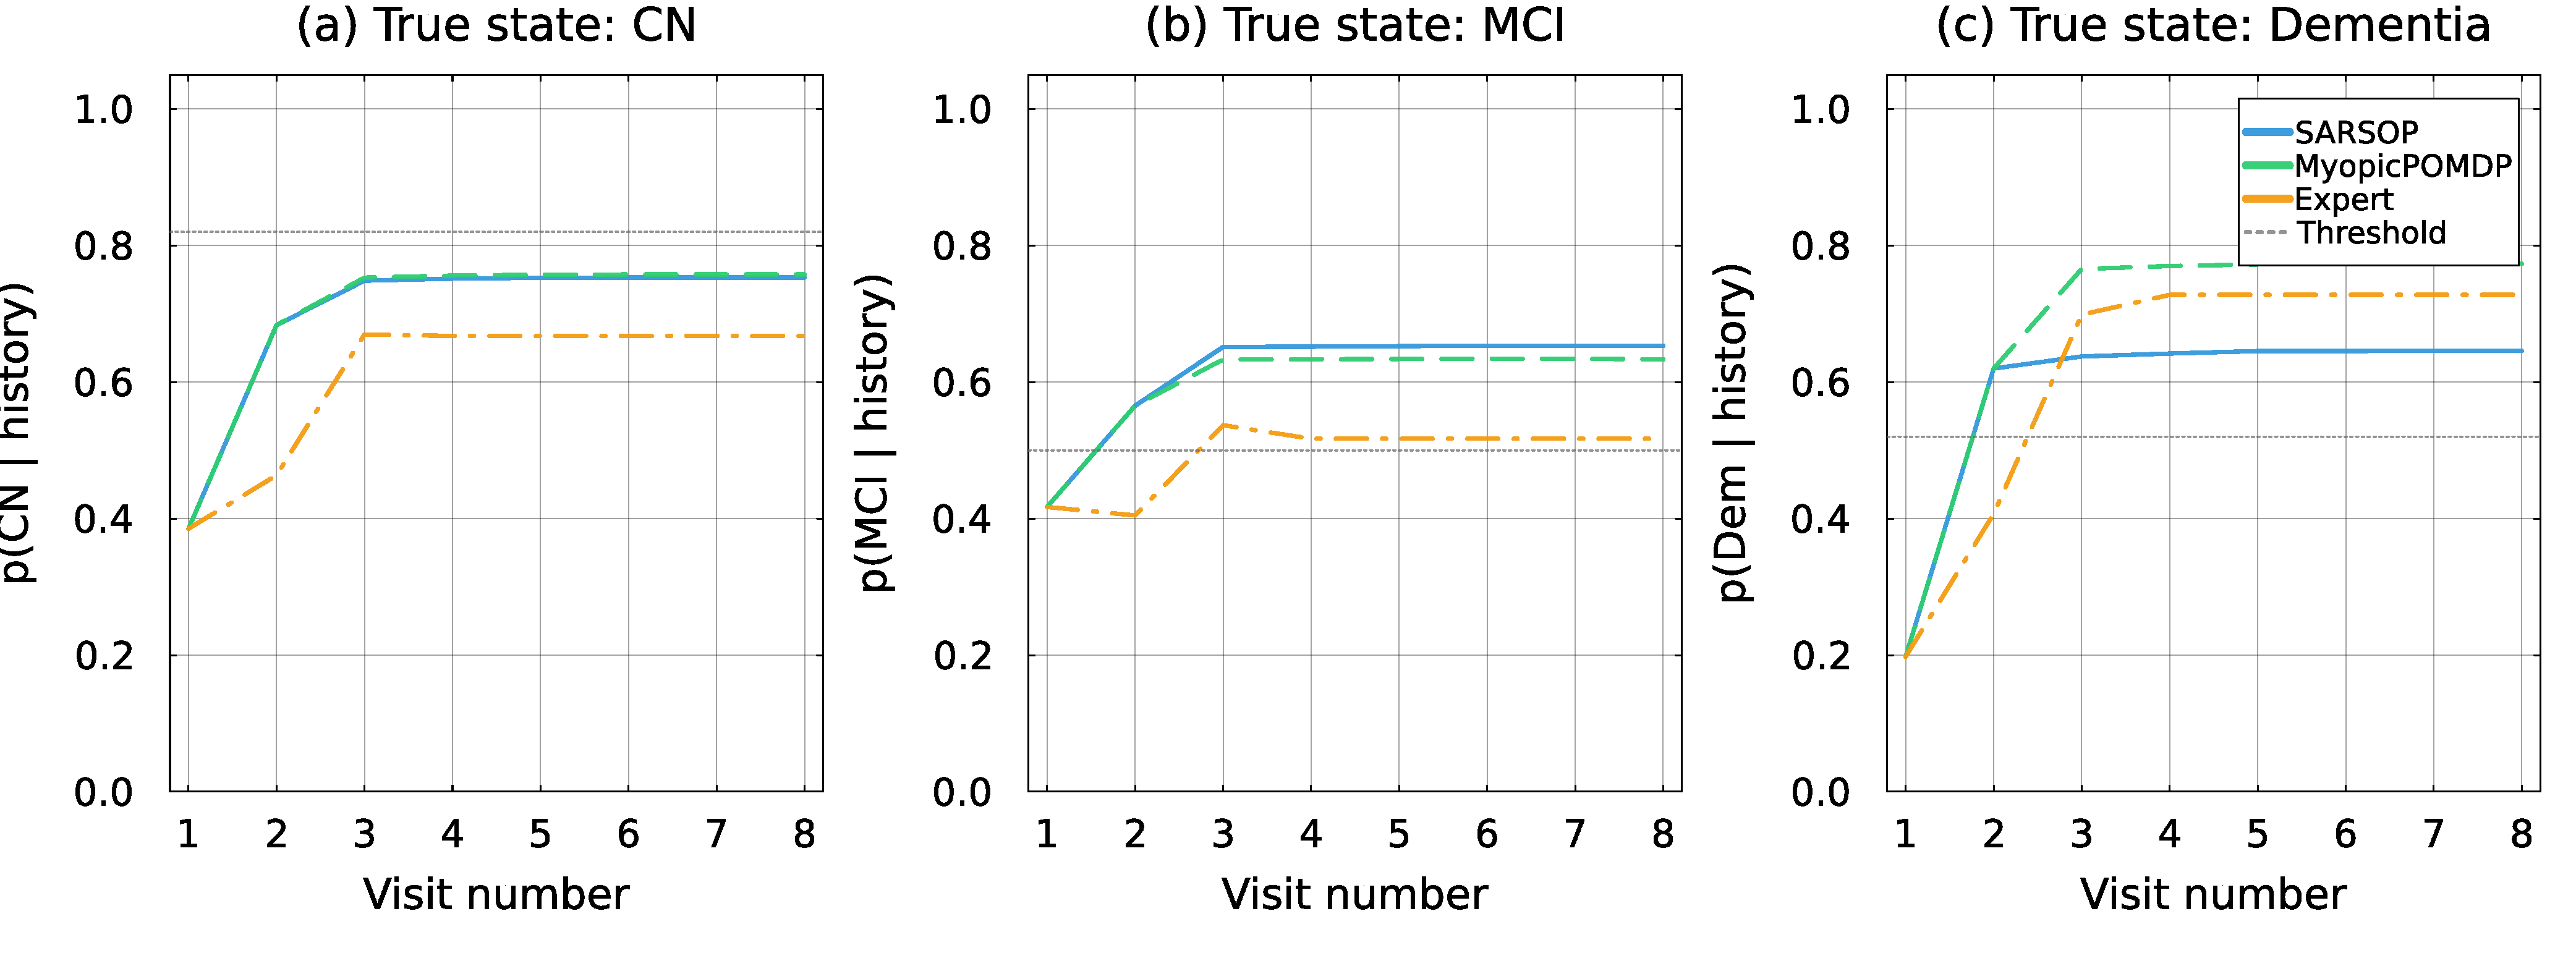
\includegraphics[width=0.76\textwidth]{figures/v2_belief_trajectory.pdf}
\caption{Average target-state belief probability (dimensionless, 0--1)
across decision visits ($N=3{,}000$ episodes per group).}
\label{fig:belief}
\end{figure*}

Fig.~\ref{fig:belief} illustrates policy-dependent belief histories.
The MCI analysis gives 2.3 versus 3.5 mean decisions for SARSOP and
Expert, compared with 2.50 versus 3.34 across all stages in
Table~\ref{tab:bench}. This is consistent with earlier commitment
under a lower utility-dependent boundary. Shared Bayesian equations
do not imply identical observation histories: chosen tests and
stopping influence the plotted averages. Reward affects belief
indirectly through those choices.

\subsection{SARSOP Policy Extraction}

We evaluated the SARSOP $\alpha$-vector policy on a uniform belief
simplex grid and grouped points by the selected action
(Table~\ref{tab:regions}, Fig.~\ref{fig:regions}). This makes the
policy's decision regions inspectable.

\begin{table}[!t]
\caption{SARSOP decision regions: fraction of the belief simplex occupied per action and minimum belief threshold for each terminal commitment. }
\label{tab:regions}
\begin{center}
\begin{tabular}{|l|c|l|}
\hline
Action & Belief\,(\%) & Min-Belief Threshold \\
\hline
Test CDR    & 79.2 & Dominant diagnostic action \\
Treat MCI   & 15.1 & $p_\mathrm{MCI} > 0.50$ \\
Treat Dem.  &  5.1 & $p_\mathrm{Dem} > 0.52$ \\
Wait        &  0.6 & $p_\mathrm{CN}  > 0.82$ \\
Test MMSE   &  0.0 & Not selected on grid \\
Test APOE4  &  0.0 & Not selected on grid \\
\hline
\end{tabular}
\end{center}
\end{table}

CDR is selected across 79.2\% of the belief space as the most
cost-effective discriminative test, while MMSE and APOE4 are never
selected: under the hand-specified MMSE model the value of information from
MMSE does not justify its cost relative to CDR, and APOE4 supplies
genetic risk rather than staging evidence. The extracted commitment
thresholds, 0.50 for MCI and 0.52 for Dementia, are far below Expert's
fixed 0.80 and 0.85, which reflects the asymmetric reward: the $-1000$
cost of failing to treat Dementia favors acting on moderate certainty.
Importantly, at the 0.50 MCI threshold the CN accuracy ($80.4{\pm}0.7\%$)
remains close to Expert's ($79.8{\pm}0.6\%$), so these results show no increase in total CN intake-stage errors in this simulation.
The minimum beliefs summarize the sampled regions; they are not
sufficient one-dimensional rules independent of the other beliefs.

\begin{figure}[!t]
\centerline{
\includegraphics[trim=0 110 0 140,clip,width=0.9\linewidth]{figures/fig10_regions.pdf}}
\caption{SARSOP policy regions over the belief simplex ($p_\mathrm{CN}$, $p_\mathrm{MCI}$, $p_\mathrm{Dem}$); CDR dominates the central diffuse region while terminal commitments occupy the belief corners. }
\label{fig:regions}
\end{figure}

\subsection{Sensitivity Analysis}
\label{sec:sensitivity}

The archived reward experiment used 1,000 episodes, seed 42, and a
five-decision cap, with SARSOP re-solved for each reward setting
(requested precision $10^{-2}$, timeout 60\,s). Its baseline overall
accuracies were 79.5\% (SARSOP) and 79.0\% (MyopicPOMDP).
Changing the Dementia-Wait utility from $-1000$ to $-500$ or $-1500$
left these accuracies unchanged to the reported precision, although
rewards changed. Doubling test costs retained SARSOP's 79.5\% but
reduced MyopicPOMDP to 73.6\%. With the MCI commitment reward reduced
from $150$ to $100$, accuracy became 79.9\% and 77.6\%, respectively.
Reward ordering was not invariant. These are separate, single-seed
stress tests rather than confidence estimates for the main benchmark.

A further observation stress test used 10,000 episodes, seed 42, and
the 20-decision cap. Replacing only the CDR MCI row
$(0.25,0.70,0.05)$ with empirical frequencies
$(0.075,0.904,0.021)$ and re-solving SARSOP gave overall accuracies of
81.6\%, 82.2\%, and 76.5\% for SARSOP, MyopicPOMDP, and Expert.
CDR remained selected at 77.9\% of 231 sampled belief points.
This supports CDR's prominence under that perturbation but also
shows that the overall accuracy ordering can reverse. The check
does not independently validate CDR or establish robustness to
joint MMSE/CDR uncertainty.

\section{Discussion}

\textbf{Transparent model integration (Contribution~1).}
Compared with prediction-focused AD models~\cite{wen2020convolutional,
grueso2021machine}, this framework makes test cost and stopping explicit.
It complements preclinical screening~\cite{onendumlu} and subtype
selection~\cite{navarro} by comparing management commitments across
CN, MCI, and Dementia. Relative to the acute stroke formulation
of~\cite{khatim}, it studies a chronic, repeated-visit setting.
Its strength is a traceable combination of empirical $T$, $b_0$, and
APOE4 with openly stated MMSE/CDR and utility assumptions. CDR's dominance in
Table~\ref{tab:regions} follows from the value of information under
the specified test costs, not from any intrinsic superiority of CDR
as an instrument.

\textbf{Subgroup and efficiency trade-offs (Contribution~2).}
The choice between episode weighting and equal-stage weighting changes
the accuracy comparison. SARSOP favors MCI intake recognition and
lower test expenditure among informed policies, whereas MyopicPOMDP
favors Dementia recognition. Because reward uses evolving states and
accuracy uses intake labels, their rankings need not coincide.
These results motivate reporting both subgroup agreement and decision
costs; they do not establish a preferred policy for clinical deployment.

\textbf{Interpretable commitment (Contribution~3).}
The extracted belief regions make the cost-information trade-off
inspectable. Earlier MCI commitment ($3.5\to2.3$ decisions in the
illustrative analysis) is consistent with a lower utility-dependent
commitment boundary, alongside policy-dependent test histories.
The difference is 1.2 decision visits, not an observed calendar-time
lead. The approach does not
demonstrate mitigation of dementia: progression is action-independent,
management actions terminate evaluation, and no post-treatment cognitive
outcome is simulated. Mitigation in the title states the intended
healthcare application, while the demonstrated contribution is a
simulation framework for investigating management delay.

\textbf{Limitations.}
Transitions are action-independent, so capturing treatment-induced
disease slowing would require data from treatment arms. The benchmark combines ADNI-estimated and hand-specified components
and evaluates them within the same simulator, so
external validation on NACC~\cite{beekly2007nacc} or
OASIS~\cite{marcus2007oasis} is needed before any clinical use. The
population-level prior $b_0$ is applied uniformly to every patient;
individualized priors could shift commitment timing. Intake-stage
agreement can penalize appropriate responses to progression and needs
comparison with decision-time staging. Transitions pool unequal visit
intervals; same-day test bundles and elapsed-time-dependent progression
are not modeled. The horizon cap and once-tested nature of APOE4
also need further assessment. Repeated APOE4 draws can overstate information. Neither
same-model simulation nor single-seed sensitivity establishes clinical
utility, observation-model validity, or general robustness.

\FloatBarrier
\section{Conclusion}

The framework combines ADNI-derived dynamics with explicit observation
and utility assumptions, compares four policies, and exposes their
belief-space decisions. Across 100,000 episodes per policy, SARSOP
and MyopicPOMDP achieve 78.3\% and 78.1\% episode-weighted
intake-stage accuracy, versus 76.6\% and 79.8\% macro accuracy.
SARSOP favors MCI recognition and lower testing expenditure among
informed policies; MyopicPOMDP favors Dementia recognition.
These conditional simulation results support further study of
management timing, but do not demonstrate slowed cognitive decline.
Future work requires decision-time evaluation, individualized priors,
persistent genetic covariates, treatment effects, and external validation.

\section*{Acknowledgments}
This work was supported by Universitas Muhammadiyah Yogyakarta.

{\footnotesize
\bibliographystyle{IEEEtran}
\bibliography{references}
}

\end{document}
